

\begin{center}

\includegraphics[scale=0.4]{01-Intro/logos/animath.jpg}
\end{center}

\vfill

Aller sur le site d'Animath (\url{https://animath.fr/actions/}) pour retrouver l’ensemble des activités de mathématiques et d’informatiques proposées.
\vfill
\vspace{4mm}

\begin{minipage}[c]{.46\linewidth}
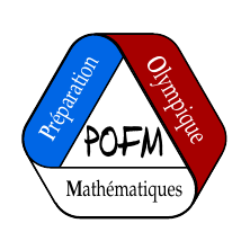
\includegraphics[width=40mm]{01-Intro/logos/pofm.png}
\end{minipage}
\begin{minipage}[c]{.46\linewidth}
\textbf{Préparation Olympique Française de Mathématiques (POFM)}.
 La sélection se fait via la Coupe Animath d'automne. La POFM organise la sélection, l’entraînement et la participation d’équipes françaises à des compétitions comme les olympiades internationales.\\
 \url{www.maths-olympiques.fr}.
\end{minipage} \hfill

\vfill
\vspace{4mm}

\vfill

\begin{minipage}[c]{.46\linewidth}

\includegraphics[width=40mm]{01-Intro/logos/tfjm.png}
\end{minipage}
\begin{minipage}[c]{.46\linewidth}
		
\textbf{TFJM}\textsuperscript{2} : un tournoi de mathématiques qui se fait en équipe (quatre à six lycéens menés par un ou deux encadrants), en proposant de travailler pendant trois mois sur des problèmes ouverts. Chaque équipe doit ensuite défendre sa solution devant d'autres équipes. \\
\url{www.tfjm.org}.
\end{minipage} \hfill

\vfill
\vspace{4mm}

\vfill


\begin{minipage}[c]{.46\linewidth}

\includegraphics[width=40mm]{01-Intro/logos/alkindi.png}
\end{minipage}
\begin{minipage}[c]{.46\linewidth}
\textbf{Concours Alkindi} : découvrez la cryptanalyse !
Concerne les classes de 4\textsuperscript{ème}, 3\textsuperscript{ème} et 2\textsuperscript{nde}. Le concours se déroule entièrement en ligne. Il est ouvert à tous et entièrement gratuit. \\
\url{ www.concours-alkindi.fr}.

\end{minipage} \hfill
\vfill
\vspace{4mm}

\vfill

\begin{minipage}[c]{.46\linewidth}

\includegraphics[width=40mm]{01-Intro/logos/utum.png}
\end{minipage}
\begin{minipage}[c]{.46\linewidth}
\textbf{«~Un texte, un mathématicien~»} :
C'est un cycle de 4 conférences pour lycéens, organisées chaque année entre janvier et avril à la Bibliothèque nationale de France. Celles-ci sont données par des chercheurs en mathématiques exceptionnels. \\
(Les vidéos des conférences sont en ligne.) \\
\url{https://animath.fr/actions/un-texte-un-mathematicien/}
\end{minipage} \hfill

\vfill
\vspace{4mm}

\pagebreak
\begin{minipage}[c]{.46\linewidth}

\includegraphics[width=40mm]{01-Intro/logos/rjm.jpg}
\end{minipage}
\begin{minipage}[c]{.46\linewidth}
\textbf{Rendez-vous des Jeunes Mathématiciennes} :
Pour les lycéennes motivées qui souhaitent s’orienter vers des études supérieures scientifiques. Passez deux ou trois jours pour s'informer des études et des carrières possibles en lien avec les mathématiques. \\
\url{www.filles-et-maths.fr}.
\end{minipage} \hfill



\vspace{4mm}



\begin{minipage}[c]{.46\linewidth}

\includegraphics[width=40mm]{01-Intro/logos/correspondances.png}
\end{minipage}
\begin{minipage}[c]{.46\linewidth}
\textbf{Correspondances de Jeunes Mathématicien·ne·s} :
Des élèves de lycée doivent réaliser, en équipe, une vidéo sur des problèmes de mathématiques. Les équipes de différents lycées s'échangent leurs vidéos, et les meilleures sont primées et diffusées. \\
\url{www.correspondances-maths.fr}.
\end{minipage} \hfill


\vspace{4mm}



\begin{minipage}[c]{.46\linewidth}

\includegraphics[width=40mm]{01-Intro/logos/clubs_de_maths.png}
\end{minipage}
\begin{minipage}[c]{.46\linewidth}	
\textbf{Clubs de mathématiques} :
Rejoignez un club pour faire des mathématiques périscolaires (olympiques ou non) ! \\
Il y en a peut-être un près de chez vous. \\
\url{https://animath.fr/actions/clubs/}

\end{minipage} \hfill

		
	
\vspace{4mm}



\begin{minipage}[c]{.46\linewidth}

\includegraphics[width=40mm]{01-Intro/logos/mathmosphere.png}
\end{minipage}
\begin{minipage}[c]{.46\linewidth}	
\textbf{Mathmosphère} : club virtuel de mathématiques.
\\
\url{https://animath.fun-campus.fr}

\end{minipage} \hfill
\vspace{16mm}

Et d'autres encore…

\vfill
		
	
\pagebreak
